\chapter{Ray tracing}
As previously hinted it is necessary to be able to simulate how radio waves
propagate through the ice for various reasons like building up a database, calibrating channels,...

It will also become necessary in the last chapter for doing actual measurements,
that's why in this chapter we'll give a brief introduction to the way radio wave
paths are found within the NuRadioMC framework.
\section{Wave propagation}
\begin{figure}[h!]
	\centering
	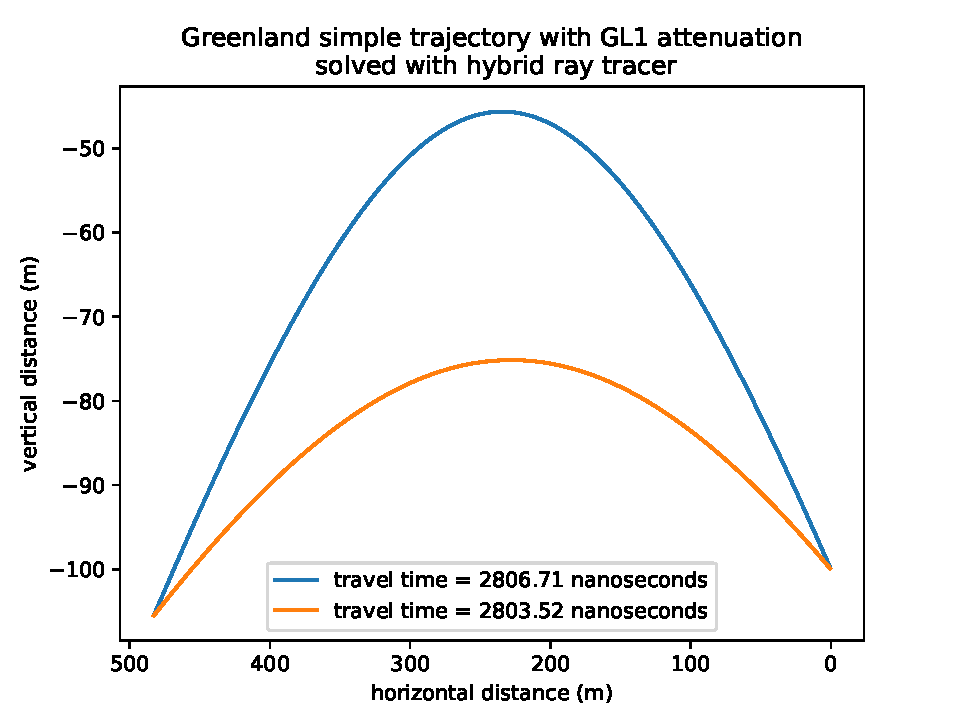
\includegraphics[width=0.7\textwidth]{path_illustration.pdf}
	\label{fig:PathIllu}
	\caption{illustration of radio wave paths generated by a neutrino event}
\end{figure}
The way we simulate the strongest waves propagating to the detector from a
radio source is through ray tracing, an illustration of such a simulation is
shown in figure \ref{fig:PathIllu}.  Here the detector is located at (0,-100)
and a radio source at (480,-108), note that there are two possible paths
leading to the detector.

The amount of solutions and how the waves are bent are consequences of the
properties of the ice we work in.  In a dielectric medium a ray propagates with
it's signal wave-speed determined by the local index of refraction as $v =
c/n$.   The effect on speed isn't the only effect the index of refraction has
which we'll need to concern ourselves with however, if a ray propagates towards
a boundary dividing 2 media with different indexes of refraction, the ray will
refract and the refracted angle can be found from Snell's law:
\begin{equation}
	n_i\sin{\theta_i} = n_o\sin{\theta_o}
\end{equation}
Where n is the index of refraction, $\theta$ the angle with respect to the
surface normal and "i" and "o" indicating incoming and outgoing respectively.
The system we'll consider however, isn't homogeneous with some specified
boundary, it's continuous: ice in Greenland has a continuously varying density and
index of refraction.

How do we know how the waves propagate in a medium?  The software we'll be
using to simulate how the radio waves behave is called \textit{Radiopropa}
\cite{Winchen_2019}. As  simulations of the wave propagation in full detail
with the finite-differences-time-domain (FDTD) technique \cite{1138693} are,
even though they are more accurate, too time consuming. The authors of
radiopropa opted to build their program on geometrical optics, i.e ray
tracing. A path of a ray $\mathbf{r}(s)$ with path parameter s in a medium
with index of refraction n($\mathbf{r}$) is described by the eikonal
equation\cite{herman2019treatise}:
\begin{equation}
	\frac{d}{ds}\left(n(\mathbf{r})\frac{d\mathbf{r}}{ds}\right) = \mathbf{\nabla} n
\end{equation}
in radiopropa the local paraxial approximation (small angle approximation) is
used, i.e if we assume that in any individual step of the algorithm the change
of the refractive index along the path $ds$ is small it's possible to re-write
the equation as:
\begin{equation}
	n(\mathbf{r})\frac{d^2\mathbf{r}}{ds^2} \approx \mathbf{\nabla} n
	\label{eqn:radiopropaformula}
\end{equation}
Which is then iteratively solved using the Cash–Karp method.  The way you would
go about using this program is thus find a start and end point (e.g a supposed
neutrino interaction point and a detector respectively), "shoot" your ray in a
certain direction for which the path will then be iteratively solved using
radiopropa. And if you chose your direction right you have the path a ray might
take from your start to the end point.  The difficulty is this direction
choosing which we'll get to later.  If there are boundaries (such as defects or
the surface) these are treated separately using Snell's law. 
\section{Ice model}
\label{section:Ice Model}
Ice has a density gradient which we'll need to account for. Due to the way the
ice bonds there will be more air trapped in between the molecules closer to the
surface than at greater depths where the pressure due to the overhead ice
prevents this.  Due to this air being trapped the density of ice will be
smaller closer to the surface than at greater depth.  

Purely from classical gravity and density considerations it can be derived that
the density scales exponentially. To see this let's consider a sheet of ice in
the Greenland firn with a surface A and a height dz, the extra pressure this
sheet of ice exerts on the ice just below it is:
\begin{equation}
	d\sigma = \frac{dF}{A} = -\frac{gdM}{A} = -g\frac{A\rho(z)dz}{A} = -g\rho(z)dz
\end{equation}
with $\rho(z)$ the depth-dependent density. Schytt assumed the
proportional change in air space to be proportional to the change in
pressure:
\begin{equation}
	\frac{dV}{V} \propto d\sigma
\end{equation}
As the volume scales inversely with the density let's assume the relation $V \propto (\rho_i - \rho)$ with
$\rho_i$ the density of pure ice, this yields\cite{herron_langway_1980}:
\begin{align}
	\frac{d\rho}{\rho_i - \rho} &\propto \rho dz\\
	\frac{d\rho}{\rho(\rho_i - \rho)} &\propto dz \label{eqn:SchyttEnd}\\
	\frac{\ln\left(\frac{\rho}{\rho_i-\rho}\right)}{\rho_i} + C &= Az\\
	\ln\left(\frac{\rho}{\rho_i-\rho}\right) &= A\rho_iz + C\\
	\frac{\rho}{\rho_i-\rho} &= e^{A\rho_iz + C} := Ae^{z/z_0}\\
	\rho &= \frac{A\rho_i e^{z/z_0}}{1 + Ae^{z/z_0}}
\end{align}
Note that Schytt worked with equation \ref{eqn:SchyttEnd} but we found
the further derivation useful. Schytt also empirically fitted the
following function:
\begin{equation}
	\label{eqn:myderiexp}
	\rho = \rho_0 e^{z/z_0} + B
\end{equation}
Figure \ref{fig:DensityMeasurements} shows how both of these
functions fit the density curve.  There is one big downside however.
It seems that the ice actually doesn't follow these exponential
curves perfectly but would more closely follow some kind of higher
order function.
\begin{figure}
  \centering
	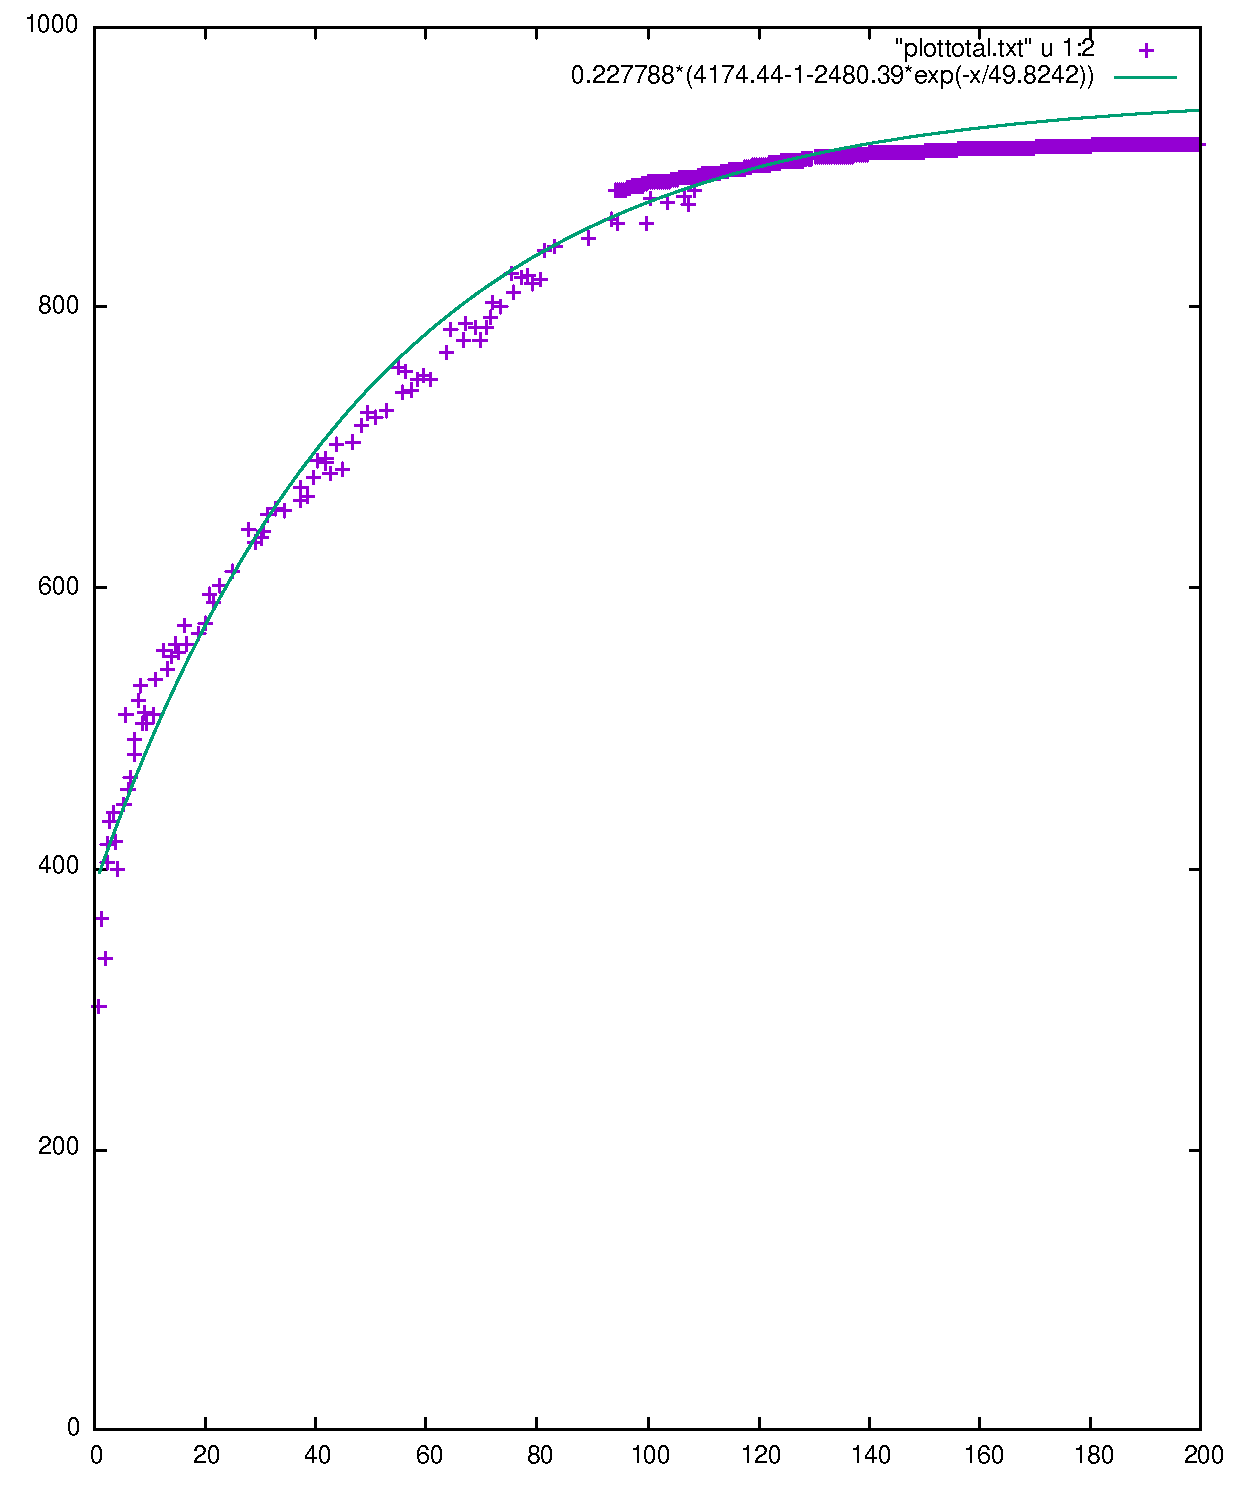
\includegraphics[width=0.5\textwidth]{Density_measurements2.pdf}
	\caption{Illustration of the shortcomings of the analytical models}
	\label{fig:DensityMeasurements}
\end{figure}

Equation \ref{eqn:radiopropaformula}, and thus the path, depends on the index
of refraction on a given location.  The dependence of the index of refraction
on density for ice can approximately be given by the Schytt equation\cite{Barwick_2018}:
\begin{equation} 
	n(x,y,z) \approx 1 + 0.78\rho(x,y,z)/\rho_0 \label{eqn:Schytt}
\end{equation} 
Where $\rho(x,y,z)$ is the local ice density and $\rho_0$ is the
density for solid ice (917 kg/m³).  For the development of the simulation
software equation \ref{eqn:myderiexp} was taken and after assuming Schytt's
equation (equation \ref{eqn:Schytt}) to hold we find that the index of refraction abides by
\begin{equation}
	\label{eqn:expn}
	n(z) = n_{ice} - \Delta n e^{z/z_0}
\end{equation}
with $n_{ice}$ the refractive index of solid ice and $\Delta n = n_{ice} - n_s$
with $n_s$ the index of refraction of snow. This exponential dependency of the
index of refraction on depth is called the \textit{single exponential model}.  

This single exponential model has a huge advantage as it's analytically
solvable, meaning that we can know which direction we'll have to shoot our ray
in (as mentioned previously) after the location of the neutrino interaction and
the detector are specified. The ray tracing algorithm developed using this
exponential index is called the \textit{analytic ray tracer}.

The discrepancy between the single exponential model and the actual data for
the density implies that the analytic ray tracer will make the wrong
predictions.  This is why the development of a different ray tracer was needed
which will be able to handle more complex ice models. One such ray tracer will
be explained in section \ref{sec:Iterative} but this ray tracer has it's
shortcomings. That's why the development of a new ray tracer was needed which
is the partial work of this thesis and we'll get to that ray tracer in chapter
\ref{chapter:hybrid}.

\begin{figure}
  \centering
  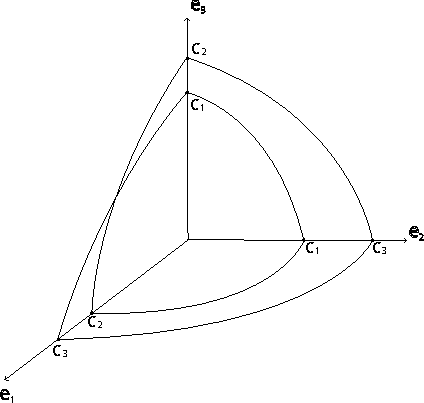
\includegraphics[width=0.5\textwidth]{figures/Fresnel.pdf}
  \caption{Wave surface of Fresnel with two sheets}
  \label{fig:Fresnel}
\end{figure}
Lastly there is an effect which might become important in the future:
birefringence.  Up until now we have implicitly assumed that ice is isotropic
meaning that both it's permittivity $\varepsilon$ and it's permeability $\mu$
are scalars but these could very well be tensorial in nature for radio waves in
ice. In general, after calculating this tensorial nature through you'd find
that in every direction two different indices of refraction can be found
implying two different types of waves each propagating with a different speed
as illustrated in figure \ref{fig:Fresnel}. Which of the two speeds in a
certain direction is then dependent on the polarization of the wave, which in
our case thus depends on the Askaryan effect (see section \ref{sec:Askaryan}).
The optical property coming from the anisotropic nature of the material is
what's called \textit{birefringence}.  Birefringence has been extensively
researched for implementation in the simulation software NuRadioMC used in the
RNO-G group \cite{Heyer2023}.
\section{Iterative ray tracer}
\label{sec:Iterative}
The iterative ray tracer \cite{2022icrc.confE1027O}, as can be derived from
it's name, iteratively searches the path a ray might take. The workings of the
first part of the explanation is illustrated in figure \ref{fig:Illustration of
iterative algorithm}.  
\begin{figure}
  \centering
  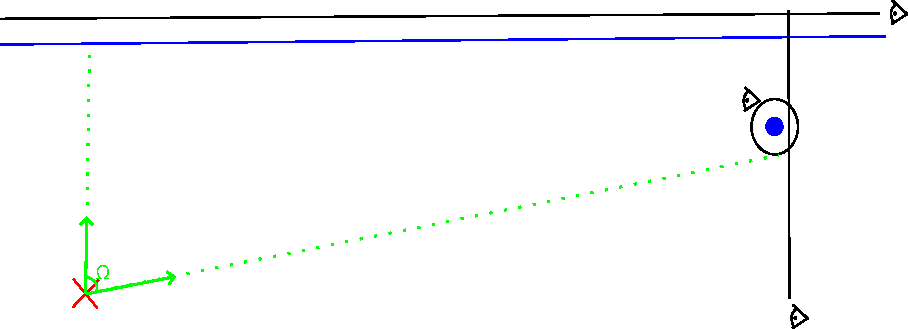
\includegraphics[width=0.7\textwidth]{algoillu.pdf}
  \caption{Illustration of the workings of the iterative algorithm}
  \label{fig:Illustration of iterative algorithm}
\end{figure}
Say we have a neutrino interaction point $\mathbf{X}_i$
(the red cross on the figure) and a detector located at $\mathbf{X}_d$ (the
blue dot on the figure), the algorithm starts by constructing an
\textit{observer} sphere with radius $r_1$ with the detector, located at $\mathbf{X}_d$, as the
center.  This means that any ray that gets shot and propagates to the sphere
will get stopped and counts as a solution.  Then, to reduce the time spent simulating, there are also observers placed
whose purpose is to stop the ray tracing but not count the observed signal as a solution.
One such observer is placed 
just above the ice surface as a ray that escapes the ice won't be able to make it back, and one
is placed just behind the detector looking from the point of the interaction vertex $\mathbf{X}_i$ as
a ray is not able to reach the detector anymore after it has passed it in the
lateral direction. 

Finally it's noted that due to the way the ice's index of refraction
continuously increases with depth, rays can't propagate upwards, this means that we only 
have to look for solutions within the angle $\Omega$ which is just the zenith angle the detector
makes with the bottom of the observer sphere.

Now that we have our setup we'll just iteratively shoot rays from the neutrino
interaction point starting at an angle $\Delta \theta_1$ then at an angle
$2\Delta \theta_1$, $3\Delta \theta_1$,... Until we have reached $\Omega$. This
process is illustrated on the left side of figure \ref{fig:IterativeWorkings}.
\begin{figure}
  \centering
  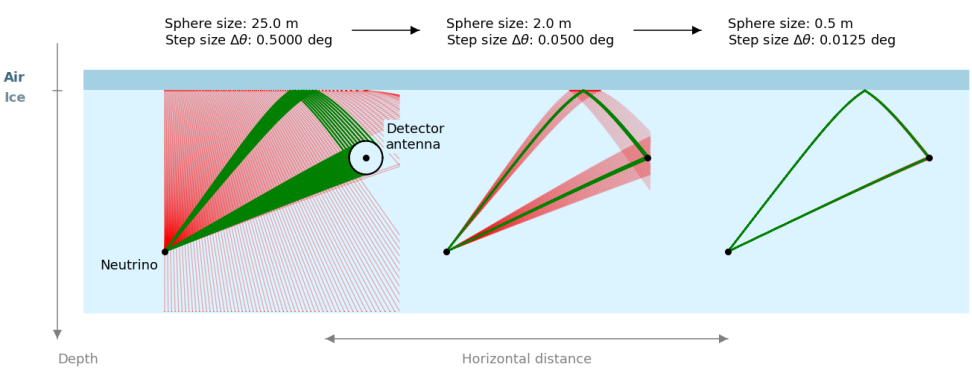
\includegraphics[width=0.7\textwidth]{IterativeWorkings.png}
  \caption{Illustration of the steps of the iterative ray tracer}
  \label{fig:IterativeWorkings}
\end{figure}
After we have gone over all the different launch angles we'll have some
solutions (marked in green) and some that don't end up on the detector (marked
in red) we can now make the observer sphere's radius smaller ($r_2 < r_1$) and
the step size of the angle smaller ($\Delta \theta_2 < \Delta \theta_1$).  And
again iteratively find the rays which end up on the sphere, only this time
looking within the angles of the solutions of the previous step. We can keep on
making the sphere and step size smaller in iterative steps until we've reached
the precision we want. We then take, for each bunch of solutions within an
angle interval, the most normal to the detector as the final solutions.



